\documentclass[
    table,
    12pt,
    oneside,
    a4paper,
    italian
]{book}

\PassOptionsToPackage{dvipsnames,table}{xcolor} % colori PDF/A + tabelle

\usepackage[table,xcdraw]{xcolor}
% PDF/A
% validate in https://www.pdf-online.com/osa/validate.aspx
\usepackage[a-1a,mathxmp]{pdfx}[2018/12/22]
\usepackage[T1]{fontenc}
\usepackage[utf8]{inputenc}
\usepackage[italian]{babel}
\usepackage{bookmark}
\usepackage{caption}
\usepackage{comment}
\usepackage{chngpage, calc} % centra il frontespizio
\usepackage{emptypage} % pagine vuote senza testatina e piede di pagina
\usepackage{epigraph} % per epigrafi
\usepackage{indentfirst} % rientra il primo paragrafo di ogni sezione
\usepackage{graphicx} % immagini
\usepackage[pdfa]{hyperref} % collegamenti ipertestuali
\usepackage{mparhack,relsize}  % finezze tipografiche
\usepackage{nameref} % visualizza nome dei riferimenti
\usepackage[font=small]{quoting} % citazioni
\usepackage{subfig} % sottofigure, sottotabelle
\usepackage[italian]{varioref} % riferimenti completi della pagina
\usepackage{longtable} % tabelle su più pagine
\usepackage[toc, acronym, automake]{glossaries}
\usepackage[backend=biber, style=verbose-ibid, hyperref, backref]{biblatex}
\usepackage{lmodern}
\usepackage[top=2.75cm, bottom=2.75cm, right=3cm, left=3.75cm]{geometry} % 1in+17pt+0.6cm
\usepackage{fancyhdr}
\usepackage{lipsum}
\usepackage{setspace}
\usepackage{titlesec}
\usepackage[cachedir=minted-caches]{minted} % https://it.overleaf.com/learn/latex/Code_Highlighting_with_minted
\usepackage{xcolor}
\usepackage{csquotes} % gestisce automaticamente i caratteri (")
\usepackage{etoolbox}
\usepackage[bottom]{footmisc}
\usepackage{zref-totpages}
% Load variables
\newcommand{\myUni}{Università degli Studi di Padova}
\newcommand{\myDepartment}{Dipartimento di Matematica ``Tullio Levi-Civita''}
\newcommand{\myFaculty}{Corso di Laurea in Informatica}
\newcommand{\myTitle}{Integrazione di Large Language Models e Data Analytics per l’Ottimizzazione delle Linee di Produzione Industriali.}
\newcommand{\myDegree}{Tesi di Laurea Triennale}
\newcommand{\profTitle}{Prof.}
\newcommand{\myProf}{Zanella Marco}
\newcommand{\graduateTitle}{Laureando}
\newcommand{\myName}{Fantinato Michael}
\newcommand{\myStudentID}{2043672}
\newcommand{\myAA}{2024-2025}
\newcommand{\myLocation}{Padova}
\newcommand{\myTime}{Luglio 2025}
% Acronyms
\newacronym{api}{API}{Application Program Interface}
\newacronym{sdk}{SDK}{Software Development Kit}
\newacronym{uml}{UML}{Unified Modeling Language}
\newacronym{tsa}{TSA}{Termine solo acronimo}
\newacronym{pmi}{PMI}{Piccole e Medie Imprese}

% Glossary
\newglossaryentry{apig}{
    name={API},
    text={Application Program Interface},
    sort=api,
    description={In informatics, an API is a set of procedures available to programmers, typically grouped to form a toolkit for a specific task within a program. Its purpose is to provide an abstraction, usually between hardware and the programmer or between low-level and high-level software, simplifying the programming process}
}

\newglossaryentry{sdkg}{
    name={SDK},
    text={Software Development Kit},
    sort=sdk,
    description={A Software Development Kit (SDK) is a collection of development tools in one installable package, facilitating application creation by providing a compiler, debugger, and sometimes a software framework. SDKs are typically specific to a hardware platform and operating system combination. Many application developers use specific SDKs to enable advanced functionalities such as advertisements, push notifications, etc}
}

\newglossaryentry{umlg}{
    name={UML},
    text={Unified Modeling Language},
    sort=uml,
    description={In software engineering, Unified Modeling Language (UML) is a modeling and specification language based on the object-oriented paradigm. UML serves as a "lingua franca" in the object-oriented design and programming community. Much of the industry literature uses UML to describe analytical and design solutions in a concise and understandable way for a broad audience}
}

\newglossaryentry{TermineSenzaAcronimo}{
    name={Nome del termine},
    sort=termine senza acronimo,
    description={Descrizione}
}

\newglossaryentry{LLM}{
    name={LLM},
    text={Large Language Model},
    sort=llm,
    description={Modello di intelligenza artificiale basato su architetture di reti neurali profonde, progettato per elaborare, comprendere e generare testo in linguaggio naturale. La loro capacità predittiva e generativa si migliora proporzionalmente alle dimensioni del modello e alla quantità di dati utilizzati durante la fase di training}
}

\newglossaryentry{API}{
    name={API},
    text={Application Programming Interface},
    sort=api,
    description={Insieme di regole, specifiche e strumenti che definiscono come i componenti software debbano interagire tra loro. Un’API espone un’interfaccia attraverso la quale un’applicazione può richiedere servizi, dati o funzionalità a un’altra, nascondendo i dettagli di implementazione interni}
}

\newglossaryentry{leadtime}{
    name={lead time},
    sort=lead time,
    description={Il termine \textit{lead time} indica l'intervallo di tempo che intercorre tra l'avvio e il completamento di un processo produttivo o logistico, utilizzato per misurare l'efficienza operativa e i tempi di risposta del sistema.}
}

\newglossaryentry{PoC}{
    name={PoC},
    text={Proof of Concept},
    sort=poc,
    description={Versione preliminare di un progetto o prototipo realizzato al fine di dimostrare la fattibilità di un’idea o di una tecnologia prima dello sviluppo completo.}
}

\newglossaryentry{KPI}{
    name={KPI},
    text={Key Performance Indicator},
    sort=kpi,
    description={Metrica quantitativa utilizzata per valutare l’efficacia di un processo o di un’attività aziendale in rapporto agli obiettivi prefissati, supportando decisioni basate su dati.}
}

\newglossaryentry{pmig}{
    name={PMI},
    text={Piccola e Media Impresa},
    sort=pmi,
    description={Impresa che, ai sensi della Raccomandazione 2003/361/CE della Commissione europea, impiega meno di 250 addetti e realizza un fatturato annuo non superiore a 50\,milioni di euro oppure un totale di bilancio annuo non superiore a 43\,milioni di euro.}
}

\makeatletter
\@ifundefined{g__tbl_row_int}{
  \expandafter\newcount\csname g__tbl_row_int\endcsname
  \csname g__tbl_row_int\endcsname=0\relax
}{}
\makeatother


% Define custom colors
\definecolor{hyperColor}{HTML}{0B3EE3}
\definecolor{tableGray}{HTML}{F5F5F7}
\definecolor{veryPeri}{HTML}{6667ab}

% Set line height
\linespread{1.5}

% Custom hyphenation rules
\hyphenation {
    data-base
    al-go-rithms
    soft-ware
}

% Images path
\graphicspath{{img/}}

% Force page color, as some editors set a grayish color as default
\pagecolor{white}

% Better spacing for footnotes
\setlength{\skip\footins}{5mm}
\setlength{\footnotesep}{5mm}

\setlength{\headheight}{14.5pt}
\addtolength{\topmargin}{-2.45pt}

% Add a subscript G to a glossary entry
\newcommand{\glox}{\textsubscript{\textbf{\textit{G}}}}

% Improvements the paragraph command
\titleformat{\paragraph}
{\normalfont\normalsize\bfseries}{\theparagraph}{1em}{}
\titlespacing*{\paragraph}
{0pt}{3.25ex plus 1ex minus .2ex}{1.5ex plus .2ex}

% Define use case environment
\newcounter{usecasecounter} % define a counter
\setcounter{usecasecounter}{0} % set the counter to some initial value
% Parameters
% #1: ID
% #2: Nome
\newenvironment{usecase}[2]{
    \renewcommand{\theusecasecounter}{\usecasename #1}  % this is where the display of the counter is overwritten/modified
    \refstepcounter{usecasecounter} % increment counter
    \vspace{2em}
    \par \noindent % start new paragraph
    {\normalsize \textbf{\usecasename #1: #2}} % display the title before the content of the environment is displayed
    \vspace{.5em}
}{
    \medskip
}
\newcommand{\usecasename}{UC}
\newcommand{\usecaseactors}[1]{\textbf{\\Attori Principali:} #1}
\newcommand{\usecasepre}[1]{\textbf{\\Precondizioni:} #1}
\newcommand{\usecasedesc}[1]{\textbf{\\Descrizione:} #1}
\newcommand{\usecasepost}[1]{\textbf{\\Postcondizioni:} #1}
\newcommand{\usecasealt}[1]{\textbf{\\Scenario Alternativo:} #1}

% Define risks environment
\newcounter{riskcounter} % define a counter
\setcounter{riskcounter}{0} % set the counter to some initial value
% Parameters
% #1: Title
\newenvironment{risk}[1]{
    \refstepcounter{riskcounter} % increment counter
    \par \noindent % start new paragraph
    \textbf{\arabic{riskcounter}. #1} % display the title before the content of the environment is displayed
    \begin{quote} % Utilizza un ambiente quote per il contenuto
}{
    \end{quote}
    \par\medskip
}
\newcommand{\riskname}{Rischio}
\newcommand{\riskdescription}[1]{\par\noindent\textbf{Descrizione:} #1.}
\newcommand{\risksolution}[1]{\par\noindent\textbf{Soluzione:} #1.}

% Apply fancy styling to pages
\pagestyle{fancy}
\fancyhf{}
\fancyhead[L]{\leftmark} % Places Chapter N. Chatper title on the top left
\fancyfoot[C]{\thepage} % Page number in the center of the footer

% Adds a blank page while increasing the page number
\newcommand\blankpage{ 
\clearpage
    \begingroup
    \null
    \thispagestyle{empty}
    \hypersetup{pageanchor=false}
    \clearpage
\endgroup
}

% Adds a blank page while increasing the page number
\newcommand\blankpagewithnumber{ 
  \clearpage
  \thispagestyle{plain} % Use plain page style to keep the page number
  \null
  \clearpage
}

% Increase page numbering
\newcommand\increasepagenumbering{
    \addtocounter{page}{+1}
}

% Make glossaries and bibliography
\makeglossaries
% Redefine the format for the glossary entries to be italic
\renewcommand*{\glstextformat}[1]{\textit{#1}\glox}
%\glsaddall

\bibliography{references/bibliography}
\defbibheading{bibliography} {
    \cleardoublepage
    \phantomsection
    \addcontentsline{toc}{chapter}{\bibname}
    \chapter*{\bibname\markboth{\bibname}{\bibname}}
}

% Code blocks handling w/ table of codes
\makeatletter
\ifdefined\NR@chapter
  \expandafter\@firstoftwo
\else
  \expandafter\@secondoftwo
\fi{\patchcmd\NR@chapter}{\patchcmd\@chapter}
  {\addtocontents{lot}{\protect\addvspace{10\p@}}}
  {\addtocontents{lot}{\protect\addvspace{10\p@}}%
   \addtocontents{lol}{\protect\addvspace{10\p@}}}
  {}{}
\makeatother

\renewcommand\listingscaption{Codice}
\renewcommand\listoflistingscaption{Elenco dei codici sorgenti}
\counterwithin*{listing}{chapter}
\renewcommand\thelisting{\thechapter.\arabic{listing}}

% Set up hyperlinks
\hypersetup{
    colorlinks=true,
    linktocpage=true,
    pdfstartpage=1,
    pdfstartview=,
    breaklinks=true,
    pdfpagemode=UseNone,
    pageanchor=true,
    pdfpagemode=UseOutlines,
    plainpages=false,
    bookmarksnumbered,
    bookmarksopen=true,
    bookmarksopenlevel=1,
    hypertexnames=true,
    pdfhighlight=/O,
    allcolors = hyperColor
}

% Set up captions
\captionsetup{
    tableposition=top,
    figureposition=bottom,
    font=small,
    format=hang,
    labelfont=bf
}

% When draft mode is on, the hyperlinks are removed. Useful when printing the document. To enable/disable, uncomment/comment the command
% \hypersetup{draft}



% Break lines in code blocks whe using inputminted
\setminted{breaklines}

\date{}

\hypersetup{pdfstartview=}
\begin{document}
    \frontmatter
    \begin{titlepage}
    \begin{center}
        \begin{Large}
            \textbf{\myUni}\\
        \end{Large}

        \vspace{5pt}

        \begin{large}
            \textsc{\myDepartment}\\
        \end{large}

        \vspace{5pt}

        \begin{large}
            \textsc{\myFaculty}\\
        \end{large}

        \vspace{25pt}
        
        \begin{figure}[htbp]
            \centering
            
\includegraphics[alt={Emblema dell'Università degli Studi di Padova}, height=6cm]{img/logo_unipd.jpeg}
        \end{figure}

        
        \begin{Large}
            \textbf{\myTitle}\\
        \end{Large}

        \vspace{5pt}

        \begin{large}
            \textit{\myDegree}\\
        \end{large}

        \vspace{50pt}
        
        \begin{normalsize}
            \begin{flushleft}
                \textit{Relatore}\\
                \profTitle\ \myProf
            \end{flushleft}

            \vspace{-48pt}
            
            \begin{flushright}
                \textit{\graduateTitle}\\
                \myName\\
                Matricola \myStudentID
            \end{flushright}
        \end{normalsize}

        \vspace*{\fill}
        
        \line(1, 0){338} \\
        \begin{normalsize}
            \textsc{Anno Accademico \myAA}
        \end{normalsize}
    \end{center}
\end{titlepage}

    \increasepagenumbering % increase the page numbrering by 1, in order to cout the frontispiece
    \clearpage
\phantomsection
\thispagestyle{empty}
\hfill
\vfill

{\small\noindent\textcopyright\ \myName, \myTime. Tutti i diritti riservati. \myDegree: ``\textit{\myTitle}'', \myUni, \myDepartment.}
    %\cleardoublepage
\phantomsection
\pdfbookmark{Ringraziamenti}{Ringraziamenti}

\begin{flushright}{
    \slshape
    ``Colui il quale ha inseguito e sconfitto i demoni Sem, che ora vagano per il mondo, domandandosi: «ma nü, chi sëm?»''} \\
    \medskip
    --- Il grande Pdor, figlio di Kmer, della tribù di Ishtar, della terra desolata dei Kfnir, uno degli ultimi sette saggi: Pfulur, Galér, Astaparigna, Sùsar, Param, Fusus e Tarìm.
\end{flushright}

\begingroup
\let\clearpage\relax
\let\cleardoublepage\relax
\let\cleardoublepage\relax

\chapter*{Ringraziamenti}

\noindent Desidero esprimere la mia gratitudine al professor \myProf, mio relatore, per l'aiuto e il sostegno che mi ha dato durante la stesura dell'elaborato.

\vspace{0.35cm}

\noindent Vorrei anche ringraziare, con affetto, i miei genitori per il loro sostegno, il grande aiuto e la loro presenza in ogni momento durante gli anni di studio.

\vspace{0.35cm}

\noindent Desidero poi ringraziare i miei amici per i bellissimi anni trascorsi insieme e le mille avventure vissute.

\vspace{0.75cm}

\noindent{\myLocation, \myTime}
\hfill \textit{\myName}

\endgroup

    \cleardoublepage
\phantomsection
\pdfbookmark{Compendio}{Compendio}
\begingroup
\let\clearpage\relax
\let\cleardoublepage\relax
\chapter*{Sommario}

La presente tesi illustra l’ideazione, la progettazione e la prototipazione di una piattaforma software 
integrata in un gestionale orientata alle \gls{pmi}, concepita per ottimizzare i processi produttivi 
attraverso un’integrazione fra servizi \textit{cloud\nobreakdash-native}, interfacce mobile e funzionalità 
di raccomandazione basate su modelli di \textit{IA}.  
L’elaborato percorre l’intero ciclo di vita del progetto: dall’analisi dei requisiti funzionali e non 
funzionali alla definizione dell’architettura, fino alla validazione sperimentale dei risultati ottenuti.

La scelta di concentrarsi su una soluzione fortemente applicativa nasce da un’esperienza maturata in 
contesti eterogenei: dapprima lavorando all’interno di una \gls{pmi} per 3 anni, quindi in una \textit{startup} impegnata 
nello sviluppo di un gestionale innovativo. In entrambe le realtà è emersa con chiarezza la necessità 
di strumenti agili, facilmente scalabili e in grado di generare valore tangibile sui flussi di lavoro 
quotidiani.  
Collaboro con \textit{Devess~S.r.l.} da oltre un anno e, proprio durante questa esperienza, 
ho concepito la funzionalità di monitoraggio intelligente descritta nella tesi.

Partendo da queste considerazioni, la tesi si propone di dimostrare la concreta fattibilità tecnica 
del prototipo realizzato con un \textit{back\nobreakdash-end} \textit{Python} e un 
\textit{front\nobreakdash-end} Flutter e la sua utilità potenziale nell’incrementare l’efficienza 
operativa. Il lavoro discute inoltre le prospettive di evoluzione futura della piattaforma e i benefici 
che un’adozione su larga scala potrebbe apportare all’ecosistema produttivo di un'azienda.

\endgroup
\vfill

    %\cleardoublepage
\pdfbookmark{\contentsname}{tableofcontents}
\setcounter{secnumdepth}{5}
\setcounter{tocdepth}{5}     

\tableofcontents
\clearpage

\begingroup
    \let\clearpage\relax
    \let\cleardoublepage\relax
    \let\cleardoublepage\relax

    % Figures list
    \phantomsection
    \pdfbookmark{\listfigurename}{lof}
    \listoffigures
    \vspace*{8ex}

    % Tables list
    \phantomsection
    \pdfbookmark{\listtablename}{lot}
    \listoftables
\endgroup

\begingroup
    % Code list
    \phantomsection
    \pdfbookmark{\listoflistingscaption}{lol}
    \listoflistings
\endgroup

\cleardoublepage
    \printglossary[type=\acronymtype, title=Acronimi e abbreviazioni, toctitle=Acronimi e abbreviazioni]
    \printglossary[type=main, title=Glossario, toctitle=Glossario]
    \blankpage % example of a blank page that also increases the page couter by 1

    \mainmatter
    % Capitolo di Introduzione — Tesi triennale di Informatica
\chapter{Introduzione}
\label{chap:introduzione}

Negli ultimi anni il settore manifatturiero è stato attraversato da una profonda trasformazione, nota con il paradigma dell’\textit{Industria~4.0}, che 
incorpora connettività diffusa, analisi dei dati in tempo reale e sistemi intelligenti di supporto alle decisioni. In questo contesto la capacità di monitorare con 
precisione le performance produttive, code ai macchinari, \gls{leadtime} e colli di bottiglia costituisce un vantaggio competitivo decisivo, soprattutto per le \gls{pmi} che puntano a ridurre gli sprechi e incrementare la flessibilità operativa.

La presente tesi nasce dalla collaborazione con l’azienda \textit{Devess~S.r.l.}, impegnata nello sviluppo di un gestionale innovativo. Durante un tirocinio di 300~ore è 
stato realizzato un \textit{proof‑of‑concept} (\gls{PoC}) di dashboard gestionale \textit{cross‑platform}, sviluppato in Flutter e sostenuto da un back‑end Python/FastAPI 
con database MongoDB, capace di integrare le \gls{API} di un \gls{LLM} per suggerire automaticamente azioni correttive o ottimizzazioni dei processi produttivi.

Per raggiungere tali traguardi è stato adottato un approccio iterativo in otto macro‑fasi settimanali, dall’onboarding tecnico al rilascio del PoC, con momenti di revisione 
periodica con il tutor aziendale. Ciascuna fase ha previsto attività di studio, sviluppo, testing e documentazione, con un focus particolare sugli algoritmi di rilevazione delle anomalie.

Oltre a costituire un contributo tangibile all’evoluzione del gestionale di Devess, il lavoro di tesi dimostra come la sinergia tra Flutter, Python e LLM abiliti soluzioni 
agili e scalabili per la \textit{smart manufacturing}, favorendo decisioni proattive e riducendo il \textit{time‑to‑action} dei responsabili di produzione.

\section{L'azienda}
Fondata nel 2020, \textit{Devess~S.r.l.} ha sede in Via Per Curnasco 58, Bergamo, e si occupa di consulenza e realizzazione di software gestionali per il settore manifatturiero. 
La piattaforma proprietaria \textit{Operativo.io} consente alle aziende di monitorare in tempo reale il flusso produttivo, analizzare li \textit{Key Performance Indicators} 
(\gls{KPI}) e intervenire prontamente in caso di inefficienze; proprio in questo software verrà implementata la nuova dashboard.

La mission di Devess è migliorare la gestione degli ordini nelle \gls{pmi}, coniugando l’esperienza dei processi produttivi tradizionali con le potenzialità offerte 
dal digitale e l'industria 4.0. L’orientamento alla \textit{data‑driven decision making} sta rendendo 
l’azienda una valida soluzione per le \gls{pmi} che desiderano intraprendere un percorso di trasformazione digitale, contenendo tempi e costi di adozione.

Durante il tirocinio il tutor aziendale, Nicola Romano, ha coordinato incontri settimanali — sia in presenza sia in modalità telematica — per monitorare l’avanzamento, fornire 
feedback puntuali e garantire l’allineamento agli obiettivi di progetto O01–O05 definiti nel piano di lavoro.

\section{L'idea}
Il progetto di stage si proponeva di sviluppare un sistema dimostrativo che integrasse analisi dati, visualizzazione interattiva e suggerimenti generati da un modello linguistico 
di grandi dimensioni. L’idea era duplice:
\begin{enumerate}
\item \textbf{Visualizzazione delle criticità}. Realizzare una dashboard che mettesse in evidenza code alle macchine, \gls{leadtime} e colli di bottiglia trovati tramite l'analisi dei dati presenti nel database MongoDB.
\item \textbf{Supporto decisionale intelligente}. Sfruttare un \gls{LLM} per suggerire, alla luce dei dati analizzati, azioni correttive concrete con potenziale estensione a un chatbot.
\end{enumerate}

La combinazione di queste componenti permette al management di individuare una criticità in pochi clic e di ricevere, contestualmente, soluzioni suggerite dall’intelligenza artificiale. Tale approccio, oltre a ridurre i tempi di analisi, favorisce una cultura operativa basata su \textit{insight} immediati e misurabili.



\section{Organizzazione del testo}
\begin{description}
    \item[{\hyperref[chap:descrizione-stage]{Il secondo capitolo}}] documenta l’impostazione operativa dello stage, le modalità di interazione con l’azienda e con il tutor, l’approccio metodologico adottato e l’analisi dei principali rischi.

    \item[{\hyperref[chap:analisi-requisiti]{Il terzo capitolo}}] presenta un’esame approfondito dei requisiti, suddivisi in obbligatori, desiderabili e opzionali, corredato dalla mappatura di attori, \textit{stakeholder}, \textit{use case} e funzionalità previste.

    \item[{\hyperref[chap:introduzione-teorica]{Il quarto capitolo}}] espone i fondamenti teorici e tecnologici alla base del progetto, confronta le soluzioni esistenti e argomenta la scelta degli strumenti impiegati.

    \item[{\hyperref[chap:lavoro-svolto]{Il quinto (ed eventuali sesto e settimo) capitolo}}] descrive in dettaglio le attività eseguite, le criticità incontrate e le soluzioni adottate, includendo schemi, tabelle e immagini ove opportuno.

    \item[{\hyperref[chap:conclusioni]{Il capitolo conclusivo}}] raccoglie le riflessioni finali: valutazione del raggiungimento degli obiettivi, competenze acquisite, possibili sviluppi futuri e considerazioni personali.
\end{description}




Riguardo alla stesura del testo, relativamente al documento sono state adottate le seguenti convenzioni tipografiche:
\begin{itemize}
  \item gli acronimi, le abbreviazioni e i termini ambigui o di uso non comune menzionati vengono definiti nel glossario, situato alla fine del presente documento;
  \item per la prima occorrenza dei termini riportati nel glossario viene utilizzata la seguente nomenclatura: \gls{apig};
  \item i termini in lingua straniera o facenti parti del gergo tecnico sono evidenziati con il carattere \textit{corsivo}.
\end{itemize}

\newpage

    % Capitolo 2 — Descrizione dello stage
\chapter{Descrizione dello stage}
\label{chap:descrizione-stage}

\section{Introduzione al progetto}

Negli ultimi anni il settore manifatturiero ha intrapreso un percorso di digitalizzazione incentrato sul paradigma dell’\textit{Industria~4.0}. In tale contesto il presente 
tirocinio, svolto presso l’azienda \textit{Devess~S.r.l.}, si propone di realizzare un \textit{proof‑of‑concept} (\gls{PoC}) da implementare in un software gestionale 
\textit{cross‑platform} sviluppato con Flutter, supportato da un back‑end \textit{Python}/FastAPI con persistenza in MongoDB e integrazione di un modello linguistico di grandi 
dimensioni (\gls{LLM}). L’obiettivo primario è consentire al management di individuare tempestivamente criticità operative, code ai macchinari, \gls{leadtime}, anomalie, colli di 
bottiglia e di ricevere suggerimenti automatici di ottimizzazione basati sui dati.

Il progetto si articola in otto macro‑fasi (cfr. sezione~\ref{subsec:pianificazione}), per un totale di 300~ore, e combina attività di analisi dati, \textit{prompt engineering}, 
sviluppo \textit{mobile} e validazione sperimentale. Il tutor aziendale, Nicola Romano, ha seguito l’avanzamento mediante allineamenti settimanali sui risultati ottenuti, 
facilitando l’accesso alle risorse necessarie.

\section{Analisi preventiva dei rischi}

\begin{risk}{Qualità dei dati in MongoDB}
\riskdescription{I dati storici potrebbero presentare valori mancanti o incoerenti, compromettendo l’accuratezza delle analisi e dei suggerimenti generati dall’intelligenza artificiale}
\risksolution{Definire procedure di \textit{data cleaning} automatizzate e introdurre controlli di validazione a campione}
\end{risk}

\begin{risk}{Costi e limiti di utilizzo delle \gls{API} LLM}
\riskdescription{L’uso intensivo delle \gls{API} di ChatGPT potrebbe superare il budget assegnato o incorrere in \textit{rate‑limit}, rendendo la funzionalità economicamente insostenibile}
\risksolution{Svolgere un’accurata analisi dei costi e monitorare i consumi del prototipo tramite \textit{dashboard} dedicata, al fine di stimare il costo medio d’utilizzo e adeguare di conseguenza il pricing del software}
\end{risk}

\begin{risk}{non-determinismo delle risposte da parte del LLM}
\riskdescription{La natura probabilistica del \gls{LLM} può produrre risposte diverse a parità di input, introducendo possibili incoerenze o inesattezze nei suggerimenti operativi}
\risksolution{Utilizzare istruzioni precise tramite \textit{prompt engineering}, e prevedere un workflow di approvazione manuale per le decisioni critiche}
\end{risk}

\begin{risk}{Scalabilità del back‑end}
\riskdescription{L’aumento del volume di dati o di richieste simultanee potrebbe ridurre le prestazioni degli endpoint FastAPI}
\risksolution{Progettare l’architettura con attenzione alla scalabilità, selezionare il deployment più adatto a un utilizzo su larga scala, adottare containerizzazione e bilanciamento del carico, prevedendo la replica del database e test di \textit{stress}}
\end{risk}

\begin{risk}{Usabilità dell’interfaccia Flutter}
\riskdescription{Un’interfaccia poco intuitiva potrebbe vanificare i benefici dell’automazione, rallentando l’adozione da parte del management}
\risksolution{Applicare le linee guida Material~3, condurre \textit{usability test} con utenti interni e iterare sulle funzionalità maggiormente critiche}
\end{risk}

\newpage

\section{Requisiti e obiettivi}

\begin{center}
    \rowcolors{1}{}{tableGray}
    \begin{tabular}{|p{2.25cm}|p{12.00cm}|}
    \hline
    \rowcolor{tableGray}\textbf{Codice} & \textbf{Descrizione} \\
    \hline
    O01 & Dashboard Flutter che visualizzi code dei macchinari, \gls{leadtime} e colli di bottiglia in tempo reale, integrata nel gestionale mobile di Devess.\\
    \hline
    O02 & Integrazione di GPT come \gls{LLM} per restituire risposte e suggerimenti in linguaggio naturale basati sui dati.\\
    \hline
    O03 & Implementazione di funzioni analitiche in grado di identificare anomalie nei processi produttivi.\\
    \hline
    O04 & Protezione dei dati sensibili con meccanismi di cifratura e controllo degli accessi basato su ruoli.\\
    \hline
    O05 & Interfaccia utente studiata in modo accurato, fruibile anche da operatori non specializzati.\\
    \hline
    D01 & Realizzazione di una versione \textit{web} dell’applicazione, integrata nel gestionale Devess.\\
    \hline
    D02 & Possibilità di interagire con un chatbot basato su \gls{LLM} per richiedere chiarimenti o soluzioni mirate.\\
    \hline
    D03 & Notifiche push o e‑mail proattive al manifestarsi di problemi o rallentamenti nella produzione.\\
    \hline
    F01 & Sincronizzazione offline con riallineamento automatico al ripristino della connettività.\\
    \hline
    F02 & Animazioni fluide e tempi di caricamento percepiti veloci.\\
    \hline
    \end{tabular}
    \captionof{table}{Requisiti e obiettivi definiti per il tirocinio.}
    \label{tab:requisiti_obbiettivi}
\end{center}

\section{Pianificazione}
\label{subsec:pianificazione}

Il lavoro è suddiviso in otto settimane; ciascuna prevede attività specifiche, \textit{milestone} e momenti di verifica con il tutor aziendale.

\begin{enumerate}
    \item \textbf{Settimana~1 — Onboarding e configurazione ambienti (40~h)}
        \begin{itemize}
            \item Configurazione degli ambienti \textit{Python}/FastAPI, Flutter e MongoDB.
            \item Studio delle \gls{API} di ChatGPT e definizione degli \textit{use case} AI.
        \end{itemize}
    \item \textbf{Settimana~2 — Prompt engineering e integrazione base LLM (40~h)}
        \begin{itemize}
            \item Applicazione di tecniche di \textit{prompt engineering}.
            \item Prima integrazione delle \gls{API} LLM con tracciamento di costi e latenza.
        \end{itemize}
    \item \textbf{Settimana~3 — Modellazione dati e MongoDB (40~h)}
        \begin{itemize}
            \item Definizione dello schema NoSQL per macchinari e produzione.
            \item Importazione e indicizzazione dei dati aziendali, con politiche di sicurezza.
        \end{itemize}
    \item \textbf{Settimana~4 — Back‑end Python e algoritmi analitici (40~h)}
        \begin{itemize}
            \item Realizzazione degli endpoint CRUD.
            \item Sviluppo degli algoritmi per code, \gls{leadtime} e colli di bottiglia.
        \end{itemize}
    \item \textbf{Settimana~5 — Validazione algoritmi e suggerimenti AI (40~h)}
        \begin{itemize}
            \item Valutazione del corretto funzionamento degli algoritmi di analisi dati.
            \item Integrazione con ChatGPT per suggerimenti contestuali.
        \end{itemize}
    \item \textbf{Settimana~6 — Automazione e performance (40~h)}
        \begin{itemize}
            \item Scheduler per analisi periodiche.
            \item Ottimizzazione delle query e monitoraggio dei costi operativi.
        \end{itemize}
    \item \textbf{Settimana~7 — UI e dashboard Flutter (40~h)}
        \begin{itemize}
            \item Progettazione del \textit{design system} secondo Material~3.
            \item Implementazione degli schermi di monitoraggio e test multi‑device.
        \end{itemize}
    \item \textbf{Settimana~8 — QA, MLOps e rilascio (20~h)}
        \begin{itemize}
            \item Test end‑to‑end e preparazione del pacchetto di rilascio.
            \item Stesura della documentazione tecnica conclusiva.
        \end{itemize}
\end{enumerate}

\subsection{Modalità di interazione con il tutor aziendale}

Sono previsti incontri di avanzamento con il tutor ogni settimana, in presenza o da remoto, per discutere le criticità emerse, verificare il rispetto del piano e concordare eventuali adeguamenti.

\subsection{Deliverable previsti}

\begin{itemize}
    \item \textbf{PoC} della dashboard gestionale completa di analisi e suggerimenti AI.
    \item Report tecnico finale strutturato nei capitoli di introduzione, architettura, metodologie, risultati e conclusioni.
    \item Codice sorgente versionato su repository Git proprietaria.
\end{itemize}

\newpage

    %--- Analisi dei requisiti ---------------------------------------------------
\chapter{Analisi dei requisiti}
\label{chap:analisi-requisiti}

\section{Casi d'uso}
Per lo studio dei casi di utilizzo del prodotto sono stati creati dei diagrammi.
I diagrammi dei casi d'uso sono diagrammi di tipo \gls{uml} dedicati alla descrizione delle funzioni o servizi offerti da un sistema, così come sono percepiti e utilizzati dagli attori che interagiscono col sistema stesso.
Di seguito i casi d'uso definitivi, suddivisi per priorità.

%--------------------------------------------------------------------------
% Casi d'uso obbligatori
%--------------------------------------------------------------------------
\subsection{Casi d'uso obbligatori}
I seguenti casi d'uso rappresentano le funzionalità fondamentali che il sistema deve necessariamente implementare per soddisfare i requisiti minimi del progetto.

\begin{figure}[htbp]
    \centering
    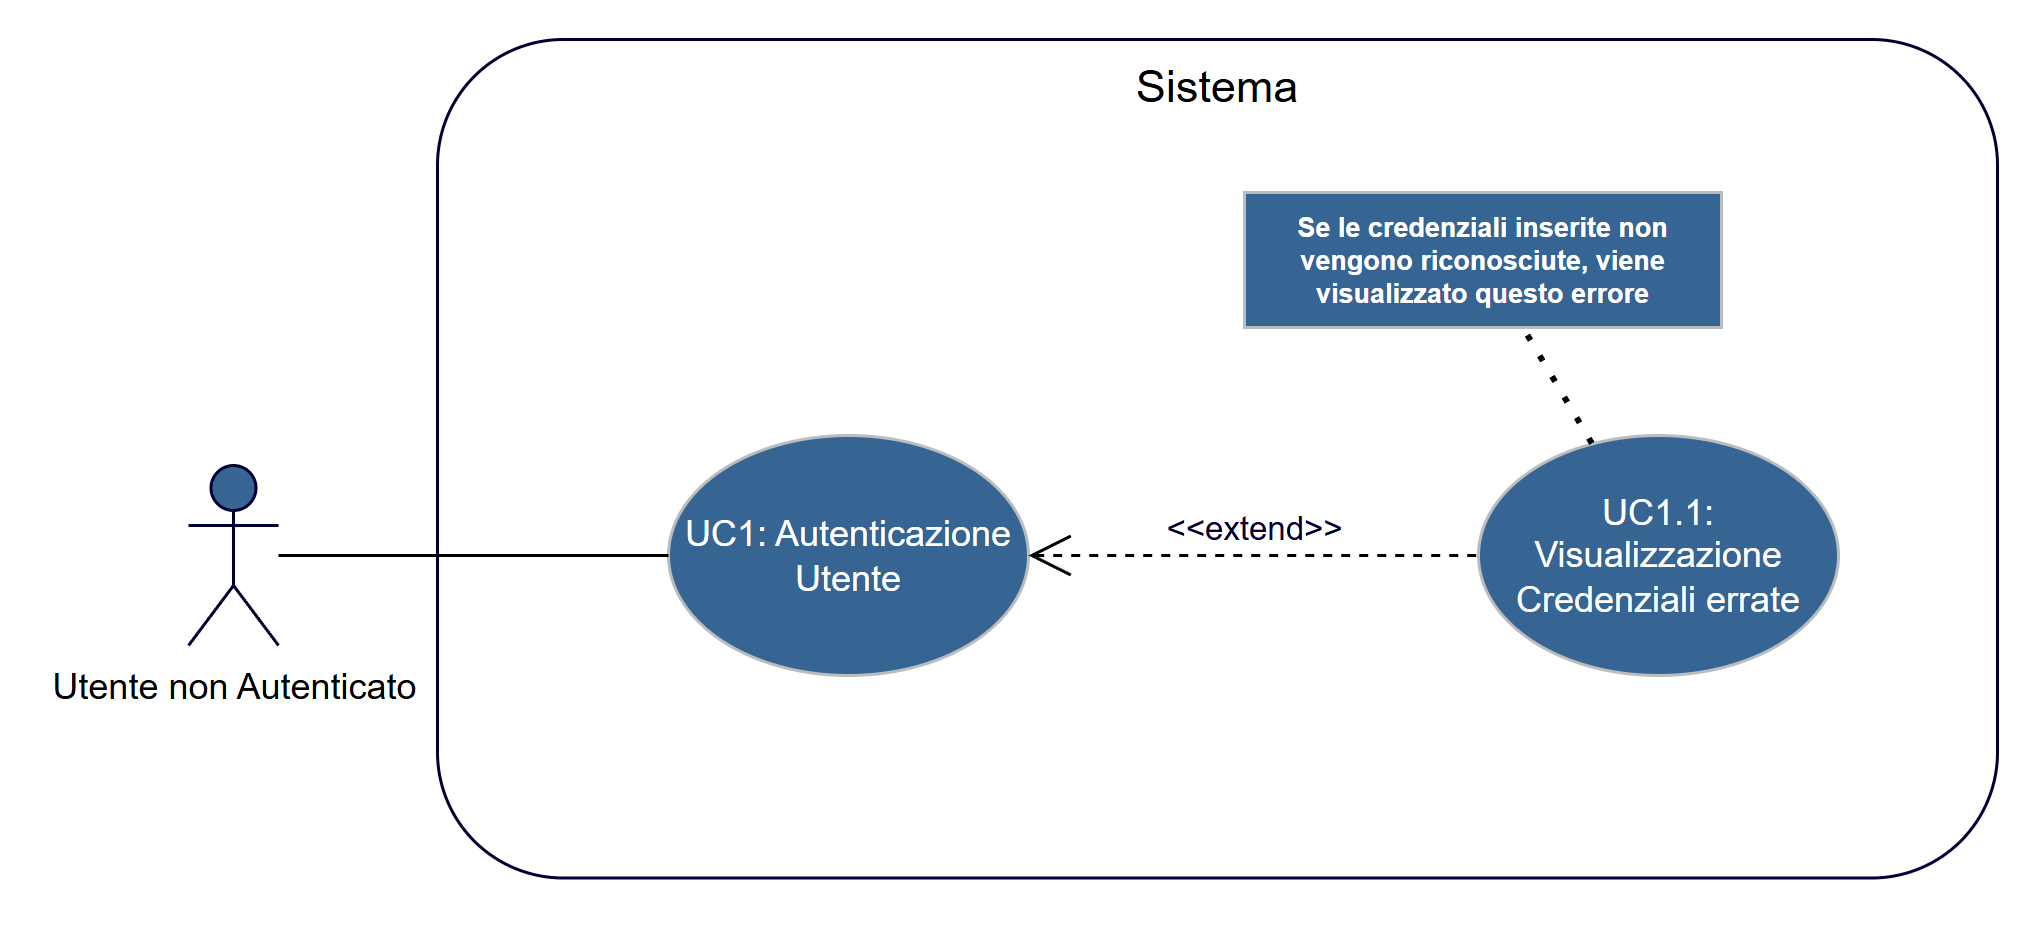
\includegraphics[alt={Diagramma UML Autenticazione Utente}, height=6cm]{img/usecase/UC1+UC1.1.png}
    \caption{UC1 + UC1.1.}
    \label{fig:uc1_login}
\end{figure}

\begin{usecase}{1}{Autenticazione Utente}
\usecaseactors{Utente non autenticato}
\usecasepre{L'utente si trova alla schermata di login.}
\usecasedesc{Il Sistema verifica le credenziali inserite e, se corrette, crea una sessione autenticata protetta.}
\usecasepost{L'utente accede alle funzionalità.}
\usecasealt{Se le credenziali non sono valide, viene mostrato un messaggio di errore (\hyperref[uc:uc1.1_errore_login]{UC1.1}).}
\label{uc:uc1_login}
\end{usecase}

\begin{usecase}{1.1}{Visualizzazione credenziali Errate}
\usecaseactors{Utente non autenticato}
\usecasepre{L'utente si trova alla schermata di login.}
\usecasedesc{Il Sistema verifica le credenziali inserite e, se scorrette, mostra un messaggio di errore.}
\usecasepost{L'utente puo riprovare reinserendo le credenziali.}
\label{uc:uc1.1_errore_login}
\end{usecase}

\begin{figure}[htbp]
    \centering
    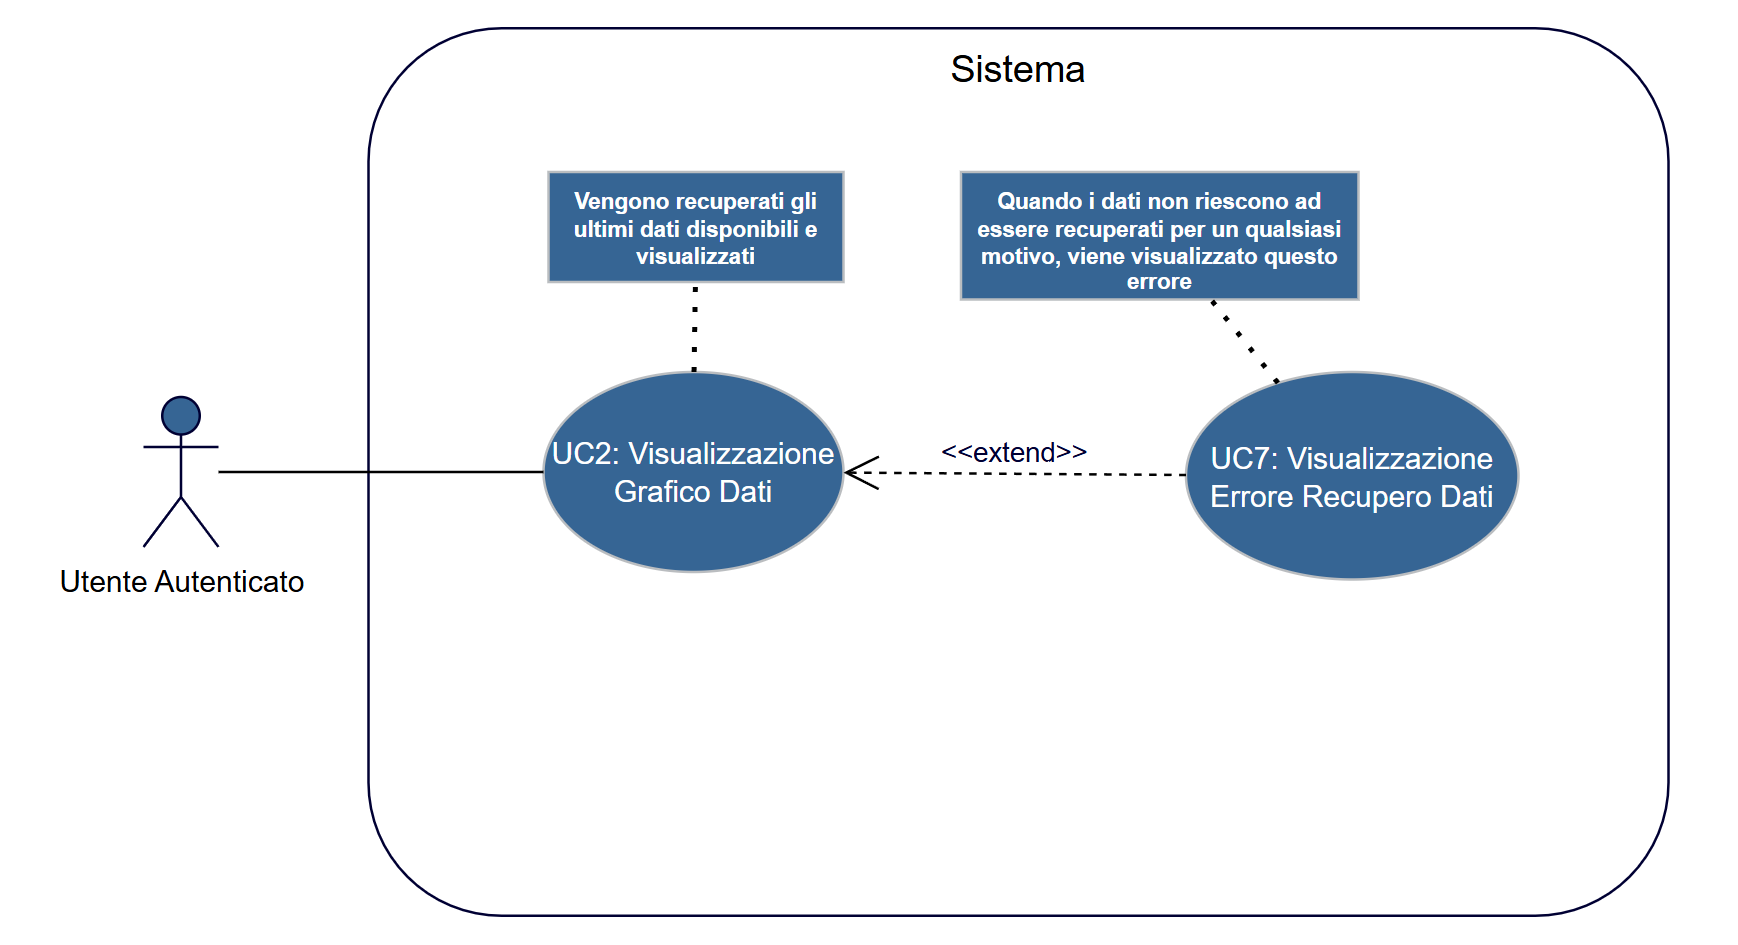
\includegraphics[alt={Diagramma UML Visualizzazione Grafico Dati}, height=7cm]{img/usecase/UC2+UC7.png}
    \caption{UC2 + UC7.}
    \label{fig:uc2_grafico}
\end{figure}

\begin{usecase}{2}{Visualizzazione Grafico Dati}
\usecaseactors{Utente}
\usecasepre{L'utente è autenticato.}
\usecasedesc{Il Sistema mostra un grafico con l'andamento temporale dei dati di produzione.}
\usecasepost{Il grafico viene aggiornato con l'ultima sincronizzazione disponibile.}
\usecasealt{Se i dati non sono presenti, viene visualizzato un messaggio di errore (\hyperref[uc:uc7_errore_dati]{UC7}).}
\label{uc:uc2_grafico}
\end{usecase}

\begin{figure}[htbp]
    \centering
    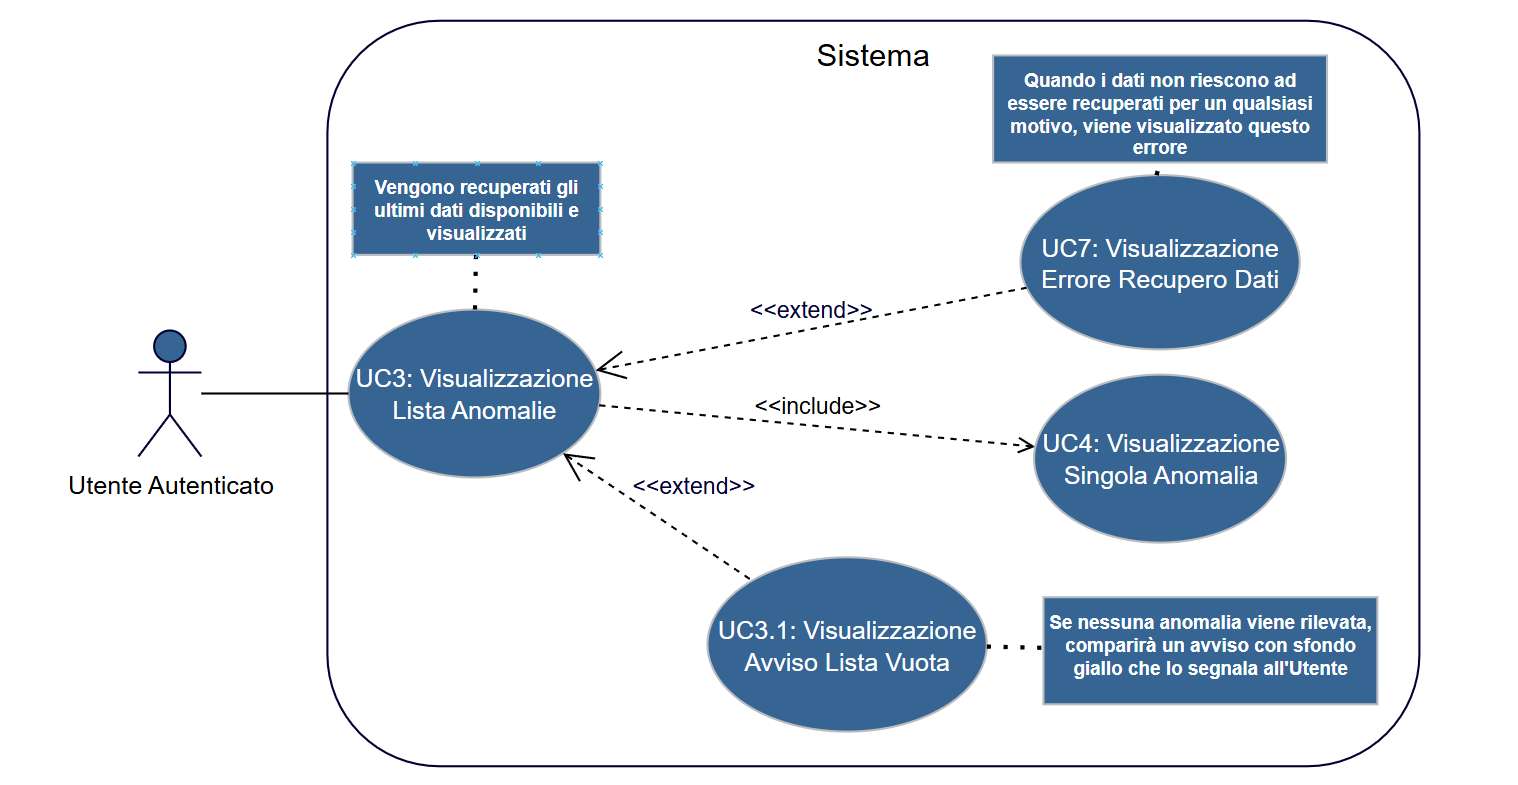
\includegraphics[alt={Diagramma UML Visualizzazione Lista Anomalie}, height=7cm]{img/usecase/UC3+UC4+UC7.png}
    \caption{UC3 + UC4 + UC7.}
    \label{fig:uc3_lista_anomalie}
\end{figure}

\begin{usecase}{3}{Visualizzazione Lista Anomalie}
\usecaseactors{Utente}
\usecasepre{Sono state eseguite analisi sui dati.}
\usecasedesc{Il Sistema elenca tutte le anomalie rilevate.}
\usecasepost{La lista è disponibile per ulteriori approfondimenti.}
\usecasealt{Se non esistono anomalie nel periodo selezionato, viene mostrato un messaggio informativo (\hyperref[uc:uc3.1_lista_anomalie_vuota]{UC3.1}).}
\usecasealt{Se il sistema non riesce a recuperare i dati viene visualizzato un errore (\hyperref[uc:uc7_errore_dati]{UC7}).}
\label{uc:uc3_lista_anomalie}
\end{usecase}

\begin{usecase}{3.1}{Visualizzazione Avviso Lista Vuota}
\usecaseactors{Utente}
\usecasepre{Sono state eseguite analisi sui dati.}
\usecasedesc{Il Sistema elenca tutte le anomalie rilevate.}
\usecasepost{Non ci sono anomalie rilevate.}
\label{uc:uc3.1_lista_anomalie_vuota}
\end{usecase}

\begin{usecase}{4}{Dettaglio Anomalia}
\usecaseactors{Utente}
\usecasepre{L'utente ha selezionato una specifica anomalia dalla lista.}
\usecasedesc{Il Sistema visualizza grafici e log di dettaglio relativi all'anomalia scelta.}
\usecasepost{L'utente può valutare la necessità di un intervento correttivo.}
\label{uc:uc4_dettaglio_anomalia}
\end{usecase}

\begin{figure}[htbp]
    \centering
    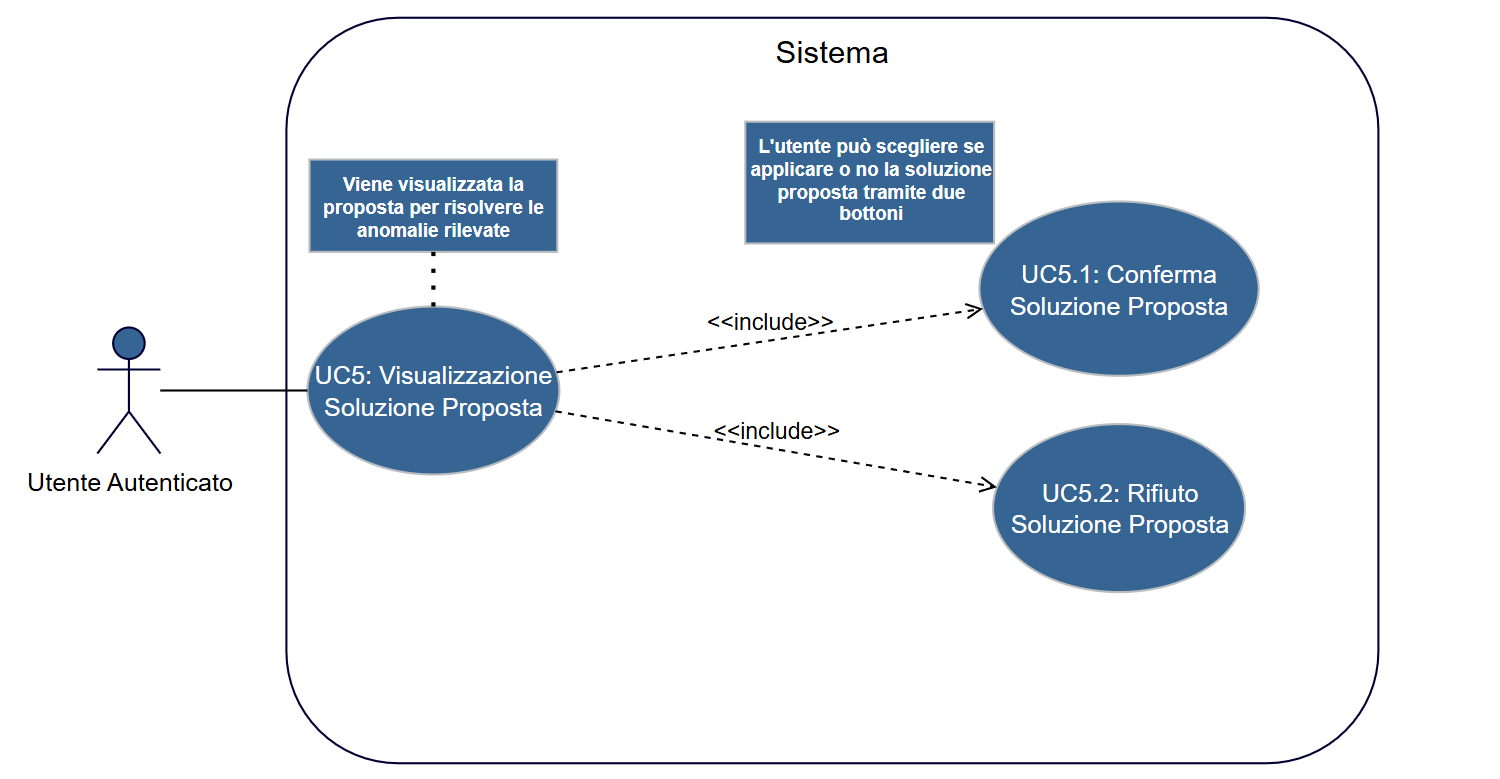
\includegraphics[alt={Diagramma UML Visualizzazione Soluzione Proposta}, height=7cm]{img/usecase/UC5+UC5.1+UC5.2.png}
    \caption{UC5 + UC5.1 + UC5.2.}
    \label{fig:uc5_soluzione_proposta}
\end{figure}

\begin{usecase}{5}{Visualizzazione Soluzione Proposta}
\usecaseactors{Utente}
\usecasepre{È stato selezionato un evento critico.}
\usecasedesc{Viene visualizzata una proposta di soluzione.}
\usecasepost{La soluzione può essere accettata (\hyperref[uc:uc5.2_conferma_soluzione]{UC5.2}) o ignorata (\hyperref[uc:uc5.1_rifiuto_soluzione]{UC5.1}).}
\label{uc:uc5_soluzione_proposta}
\end{usecase}

\begin{usecase}{5.1}{Rifiuto Soluzione Proposta}
\usecaseactors{Utente}
\usecasepre{È visualizzata una soluzione proposta (\hyperref[uc:uc5_soluzione_proposta]{UC5}).}
\usecasedesc{L'Utente rifiuta la soluzione proposta.}
\usecasepost{Il sistema registra il rifiuto e mantiene l'anomalia aperta.}
\label{uc:uc5.1_rifiuto_soluzione}
\end{usecase}

\begin{usecase}{5.2}{Conferma Soluzione Proposta}
\usecaseactors{Utente}
\usecasepre{È visualizzata una soluzione proposta (\hyperref[uc:uc5_soluzione_proposta]{UC5}).}
\usecasedesc{L'Utente approva la soluzione che viene applicata al sistema di produzione.}
\usecasepost{Il sistema avvia l'esecuzione del piano correttivo.}
\label{uc:uc5.2_conferma_soluzione}
\end{usecase}

\begin{figure}[htbp]
    \centering
    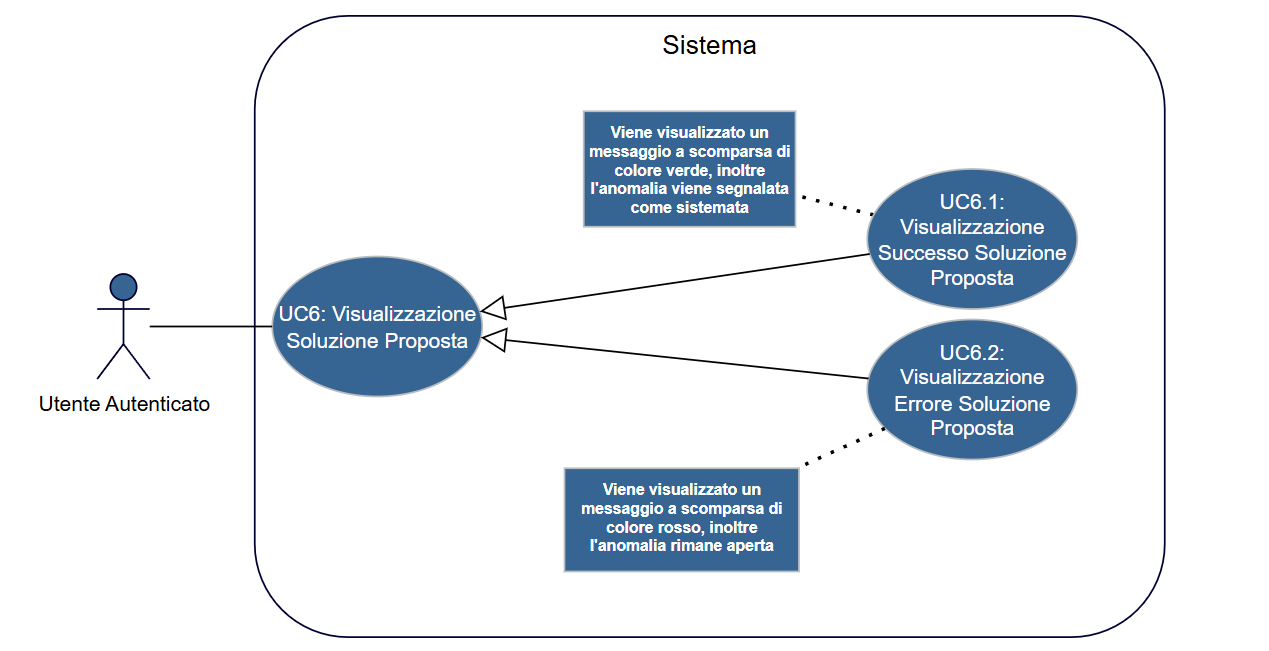
\includegraphics[alt={Diagramma UML Visualizzazione Soluzione Proposta}, height=7cm]{img/usecase/UC6+UC6.1+UC6.2.png}
    \caption{UC6 + UC6.1 + UC6.2.}
    \label{fig:uc6_visualizzazione_soluzione}
\end{figure}

\begin{usecase}{6}{Visualizzazione Soluzione Proposta}
\usecaseactors{Utente}
\usecasepre{Il piano correttivo è stato approvato ed eseguito.}
\usecasedesc{Il Sistema notifica all'Utente il risultato.}
\usecasepost{In base al successo o no dell'applicazione, il messaggio puo essere positivo (\hyperref[uc:uc6.1_soluzione_ok]{UC6.1}) o negativo(\hyperref[uc:uc6.2_soluzione_err]{UC6.2}).}
\label{uc:uc6_visualizzazione_soluzione}
\end{usecase}

\begin{usecase}{6.1}{Visualizzazione Successo Soluzione Proposta}
\usecaseactors{Utente}
\usecasepre{Il piano correttivo è stato eseguito correttamente.}
\usecasedesc{Il Sistema notifica all'Utente l'avvenuta applicazione della soluzione.}
\usecasepost{L'anomalia viene marcata come risolta.}
\label{uc:uc6.1_soluzione_ok}
\end{usecase}

\begin{usecase}{6.2}{Visualizzazione Errore Soluzione Proposta}
\usecaseactors{Utente}
\usecasepre{Il sistema ha tentato di applicare una soluzione proposta.}
\usecasedesc{Il Sistema segnala all'Utente il fallimento dell'applicazione e fornisce i dettagli dell'errore.}
\usecasepost{L'anomalia resta aperta e viene registrato il tentativo fallito.}
\label{uc:uc6.2_soluzione_err}
\end{usecase}

\begin{usecase}{7}{Visualizzazione Errore Recupero Dati}
\usecaseactors{Utente}
\usecasepre{L'utente è autenticato.}
\usecasedesc{Il Sistema mostra un errore perché i dati non sono presenti.}
\usecasepost{l'utente può aggiornare la pagina per riprovare a recuperare i dati.}
\label{uc:uc7_errore_dati}
\end{usecase}

%--------------------------------------------------------------------------
% Casi d'uso desiderabili
%--------------------------------------------------------------------------
\subsection{Casi d'uso desiderabili}
I seguenti casi d'uso rappresentano le funzionalità desiderabili che il sistema potrebbe implementare per migliorare l'esperienza dell'utente e fornire funzionalità aggiuntive.

\begin{figure}[htbp]
    \centering
    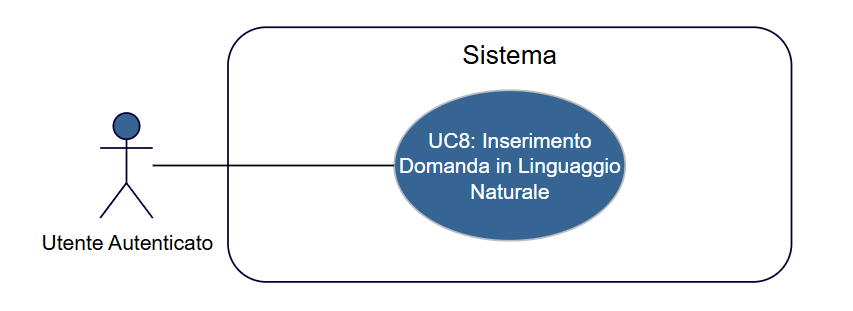
\includegraphics[alt={Diagramma UML Inserimento Domanda in Linguaggio Naturale}, height=5cm]{img/usecase/UC8.png}
    \caption{UC8.}
    \label{fig:uc8_domanda_nl}
\end{figure}

\begin{usecase}{8}{Inserimento Domanda in Linguaggio Naturale}
\usecaseactors{Utente}
\usecasepre{L'utente è autenticato.}
\usecasedesc{L'utente inserisce una domanda libera relativa al sistema.}
\usecasepost{La domanda viene inoltrata al \gls{LLM}.}
\label{uc:uc8_domanda_nl}
\end{usecase}

\begin{figure}[htbp]
    \centering
    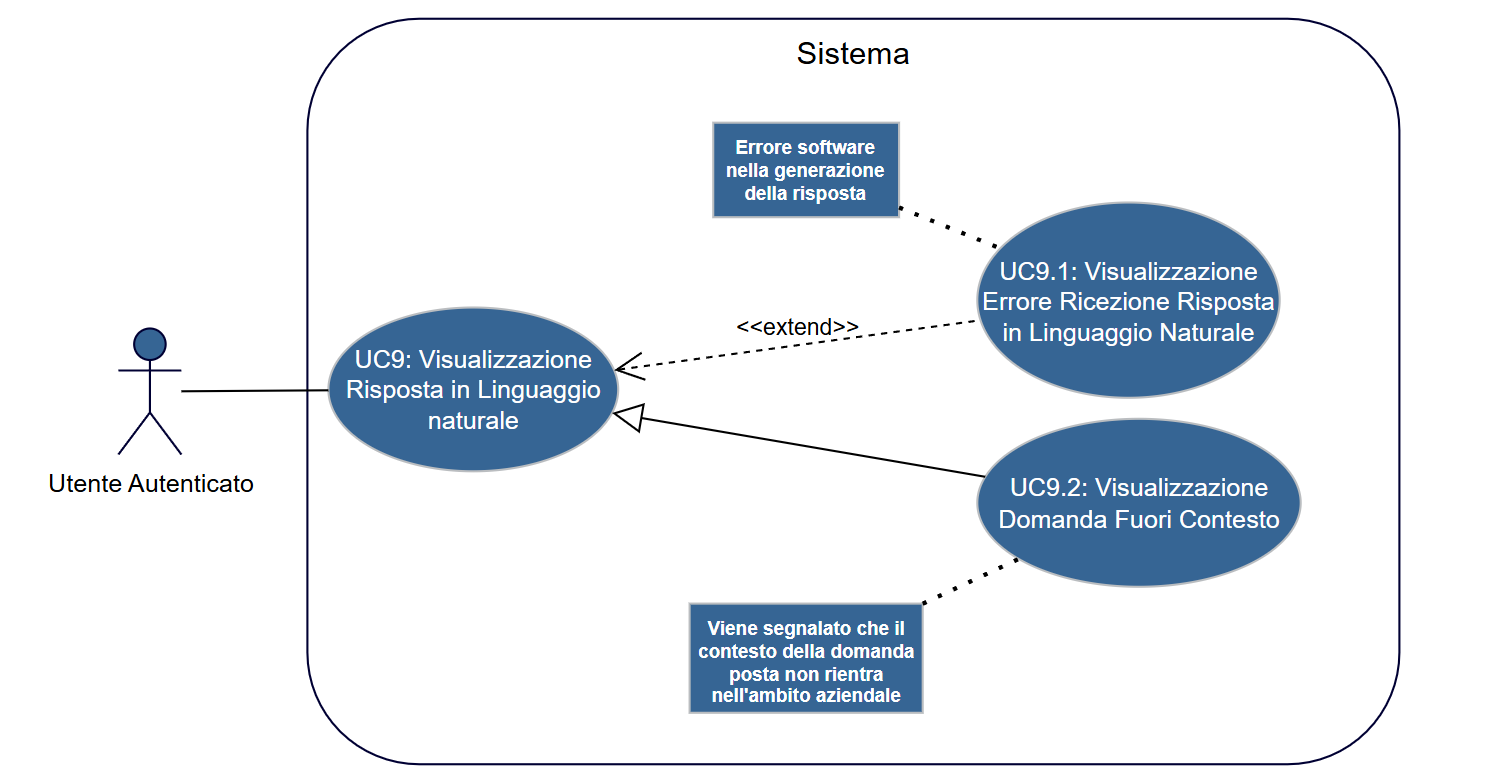
\includegraphics[alt={Diagramma UML Visualizzazione Risposta in Linguaggio Naturale}, height=7cm]{img/usecase/UC9+UC9.1+UC9.2.png}
    \caption{UC9 + UC9.1 + UC9.2.}
    \label{fig:uc9_risposta_nl}
\end{figure}

\begin{usecase}{9}{Visualizzazione Risposta in Linguaggio Naturale}
\usecaseactors{Utente}
\usecasepre{È stata inoltrata una domanda (\hyperref[uc:uc8_domanda_nl]{UC8}).}
\usecasedesc{Viene visualizzata una risposta generata in linguaggio naturale.}
\usecasepost{La risposta è visualizzata all'Utente.}
\usecasealt{Se si verifica un errore, viene mostrato un messaggio di errore (\hyperref[uc:uc9.1_errore_nl]{UC9.1}).}
\usecasealt{Se la domanda è fuori contesto, il Sistema chiede all'utente di riformulare (\hyperref[uc:uc9.2_fuori_contesto_nl]{UC9.2}).}
\label{uc:uc9_risposta_nl}
\end{usecase}

\begin{usecase}{9.1}{Visualizzazione errore ricezione risposta in linguaggio naturale}
\usecaseactors{Utente}
\usecasepre{È stata inoltrata una domanda (\hyperref[uc:uc8_domanda_nl]{UC8}).}
\usecasedesc{Il sistema non riesce a recuperare la risposta.}
\usecasepost{L'utente visualizza un errore che lo informa del problema.}
\label{uc:uc9.1_errore_nl}
\end{usecase}

\begin{usecase}{9.2}{Visualizzazione domanda fuori contesto}
\usecaseactors{Utente}
\usecasepre{È stata inoltrata una domanda (\hyperref[uc:uc8_domanda_nl]{UC8}) non inerente all'ambito operativo.}
\usecasedesc{L'utente visualizza un avviso che la domanda posta era fuori contesto.}
\usecasepost{L'utente può riformulare la domanda.}
\label{uc:uc9.2_fuori_contesto_nl}
\end{usecase}

\begin{figure}[htbp]
    \centering
    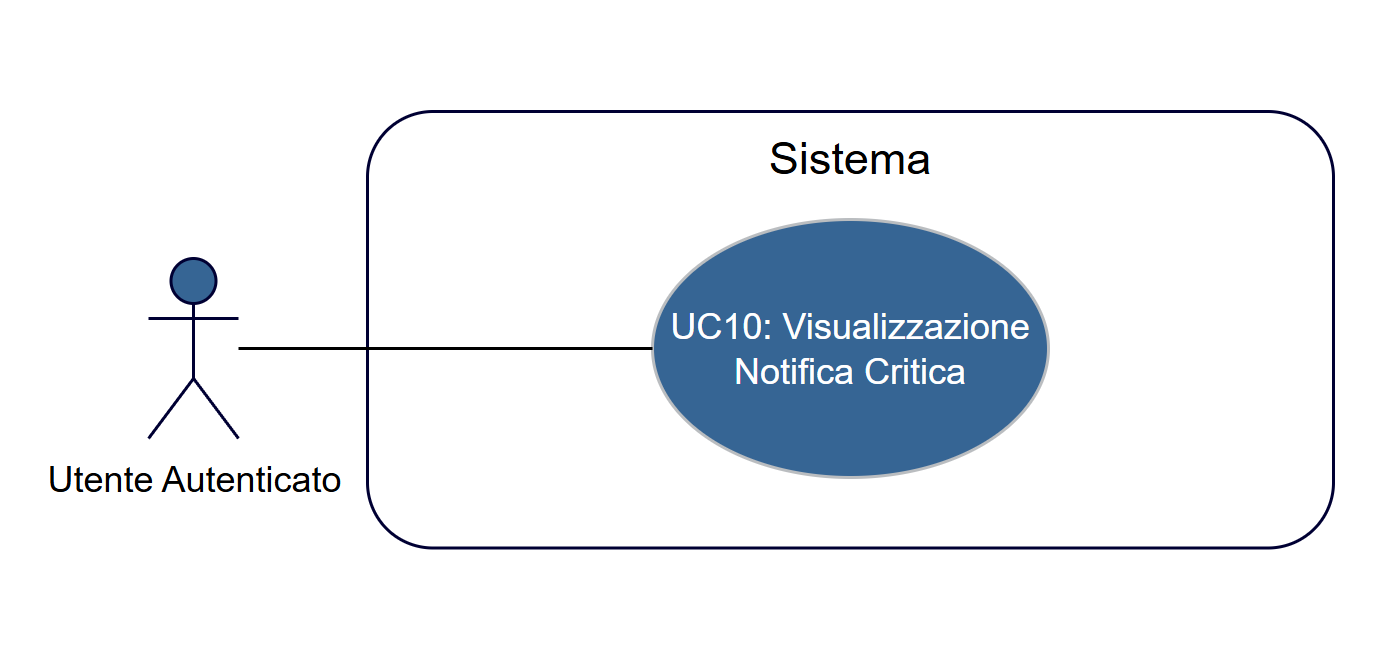
\includegraphics[alt={Diagramma UML Visualizzazione Notifica Critica}, height=5cm]{img/usecase/UC10.png}
    \caption{UC10.}
    \label{fig:uc10_notifiche}
\end{figure}


\begin{usecase}{10}{Visualizzazione Notifica Critica}
\usecaseactors{Utente}
\usecasepre{Il sistema rileva un'anomalia critica.}
\usecasedesc{Viene visualizzato un avviso sui dispositivi connessi.}
\usecasepost{Gli operatori visualizzano l'avviso.}
\label{uc:uc10_notifiche}
\end{usecase}

%--------------------------------------------------------------------------
% Casi d'uso facoltativi
%--------------------------------------------------------------------------
\subsection{Casi d'uso facoltativi}
I seguenti casi d'uso rappresentano le funzionalità facoltative che il sistema potrebbe implementare per migliorare l'esperienza dell'utente e fornire funzionalità aggiuntive.

\begin{figure}[htbp]
    \centering
    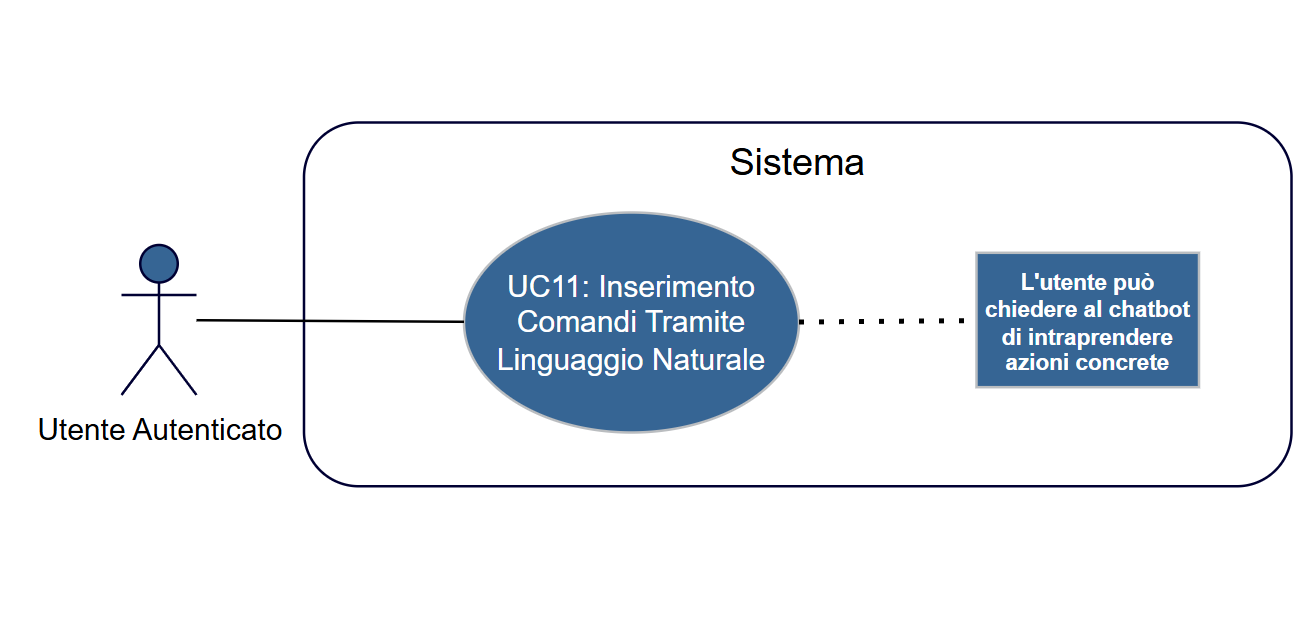
\includegraphics[alt={Diagramma UML Inserimento Comandi Tramite Linguaggio Naturale}, height=5cm]{img/usecase/UC11.png}
    \caption{UC11.}
    \label{fig:uc11_comandi_nl}
\end{figure}

\begin{usecase}{11}{Inserimento Comandi Tramite Linguaggio Naturale}
\usecaseactors{Utente}
\usecasepre{L'utente è autenticato e l'interfaccia dei comandi NL è attiva.}
\usecasedesc{L'utente impartisce comandi operativi in linguaggio naturale; il Sistema li interpreta e li esegue.}
\usecasepost{L'azione richiesta viene completata o ne viene comunicato l'esito.}
\label{uc:uc11_comandi_nl}
\end{usecase}

%--------------------------------------------------------------------------
% Tracciamento dei requisiti
%--------------------------------------------------------------------------
\section{Tracciamento dei requisiti}
Il tracciamento mostra la copertura dei requisiti funzionali (F) classificati come
\textbf{N} (obbligatori), \textbf{D} (desiderabili) e \textbf{Z} (facoltativi).

\begin{center}
  \brandTableColors
  \begin{longtable}{|p{2.25cm}|p{7.75cm}|p{2.25cm}|}
    \hline
    \multicolumn{1}{|c|}{\textbf{Requisito}} &
    \multicolumn{1}{c|}{\textbf{Descrizione}} &
    \multicolumn{1}{c|}{\textbf{Use Case}}\\
    \hline
    FN1 & Login sicuro dell'utente                                    & UC1, UC1.1 \\ \hline
    FN2 & Visualizzare grafico dei dati di produzione                 & UC2, UC7   \\ \hline
    FN3 & Elencare le anomalie rilevate                               & UC3, UC3.1, UC7 \\ \hline
    FN4 & Mostrare il dettaglio di una anomalia                       & UC4        \\ \hline
    FN5 & Presentare una soluzione proposta tramite LLM               & UC5, UC5.1, UC5.2 \\ \hline
    FN6 & Gestire l'accettazione/rifiuto di una soluzione             & UC5.1, UC5.2 \\ \hline
    FN7 & Notificare risultato applicazione soluzione                 & UC6, UC6.1, UC6.2 \\ \hline
    FN8 & Gestire errori di recupero dati                             & UC7        \\ \hline
    FD1 & Inserire domande in linguaggio naturale                     & UC8        \\ \hline
    FD2 & Ricevere risposte in linguaggio naturale                    & UC9, UC9.1, UC9.2 \\ \hline
    FD3 & Visualizzare notifiche critiche                             & UC10       \\ \hline
    FZ1 & Inserire comandi in linguaggio naturale                     & UC11       \\ \hline
  \end{longtable}
  \captionof{table}{Tracciamento dei requisiti funzionali.}
  \label{tab:requisiti_fun}
\end{center}


    %\chapter{Introduzione}
\label{chap:introduzione-teorica}
    %\chapter{Introduzione}
\label{chap:lavoro-svolto}
    %\chapter{Conclusioni}
\label{chap:conclusioni}

\section{Consuntivo finale}
Esempio di aggiunta di un termine con glossario e acronimo:\\
Lorem \gls{sdk} ispum dolor.

Nel successivo utilizzo, apparirà solo l'acronimo:\\
Lorem \gls{sdk}.

Nel caso si voglia invece mettere solo il termine per esteso, si può usare:\\
Lorem \gls{sdkg}.

\section{Raggiungimento degli obiettivi}
Esempio di termine con solo acronimo\\
Lorem \gls{tsa}, ipsum dolor sit amet

termine costruito senza acronimo:
Lorem \gls{TermineSenzaAcronimo}, ipsum dolor sit amet

\section{Conoscenze acquisite}
Lorem Ipsum dolor Lorem \gls{api}

Lorem Ipsum dolor Lorem \gls{apig}

Si può consultare il file \textit{glossary\_acronyms.tex} per alcuni esempi.

\section{Valutazione personale}


\section{Valutazione personale}


\newpage

    \pagenumbering{roman}
    \backmatter
    %\chapter{Bibliografia}
\label{cap:bibliography}

\nocite{*}

% Books bibliography
\printbibliography[heading=subbibliography, title={Testi}, type=book]

% Articles bibliography
\printbibliography[heading=subbibliography, title={Articoli}, type=article]

% Websites bibliography
%\printbibliography[heading=subbibliography, title={Siti}, type=online]

    %\chapter{Sitografia}
\label{cap:webliography}
\nocite{*}

% Websites bibliography
\printbibliography[heading=subbibliography, title={\null}, type=online]

\end{document}